\subsection{拉伸构建垫片三维建模}
\begin{procedure}
\item关闭“中心线”层,关闭后的结果如图\ref{fig:offcenterlayer}所示。图层的关闭方法有:
\begin{itemize}
\item 单击【工具栏】中的
\includegraphics[scale=0.6]{layercontral.png}图标,从弹出列表中点击“中心线”层中的
\includegraphics[scale=0.6]{layeronoffset.png}图标,使其变为
\includegraphics[scale=0.6]{layeroffstatus.png}灰色状态。
\item 打开【图层特性管理器,点击“中心线”层中的
\includegraphics[scale=0.6]{layeronoffset.png}图标,使其变为
\includegraphics[scale=0.6]{layeroffstatus.png}灰色状态。
\end{itemize}
\item 通过拉伸操作构建圆柱体,拉伸结果如图\ref{fig:dianpianextrude}所示。
\begin{lstlisting}
|命令: EXTRUDE|
|当前线框密度:  ISOLINES=4,闭合轮廓创建模式 = 实体|
|选择要拉伸的对象或 [模式(MO)]: 指定对角点: 找到 8 个|
|选择要拉伸的对象或 [模式(MO)]:|
|指定拉伸的高度或 [方向(D)/路径(P)/倾斜角(T)/表达式(E)]: 2|
\end{lstlisting}
\item 切换视图为西南等轴测图。点击【视图】菜单中【三维视图】子菜单中的【西南等轴测】。
\item 进行差集操作,构建垫片的三维模型
\begin{lstlisting}
|命令: subtract |
|选择要从中减去的实体、曲面和面域...|
|选择对象: 找到 1 个|
|选择对象:  选择要减去的实体、曲面和面域...|
|选择对象: 找到 1 个|
|选择对象: 找到 1 个,总计 2 个|
|选择对象: 找到 1 个,总计 3 个|
|选择对象: 找到 1 个,总计 4 个|
|选择对象: 找到 1 个,总计 5 个|
|选择对象: 找到 1 个,总计 6 个|
|选择对象: 找到 1 个,总计 7 个|
|选择对象:|
\end{lstlisting}
\begin{figure}[htbp]
\centering
\subfloat[]{\label{fig:offcenterlayer}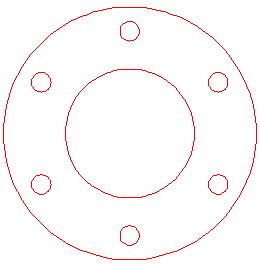
\includegraphics[scale=0.2]{offcenterlayer.png}}\hspace{20pt}
\subfloat[]{\label{fig:dianpianextrude}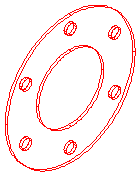
\includegraphics[scale=0.3]{dianpianextrude.png}}\hspace{20pt}
\subfloat[]{\label{fig:dianpiansolid}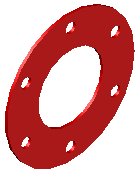
\includegraphics[scale=0.3]{dianpiansolid.png}}
\caption{垫片拉伸建模过程}
\end{figure}
\item 设置视觉样式为真实,其结果如图\ref{fig:dianpiansolid}所示。设置方法为:点击【视图】菜单中【视觉样式】子菜单中的【真实】项。
\item 将垫片模型保存为“调压阀垫片立体图.dwg”。
\end{procedure}
